\chapter{Chapter ~\ref{ch:modeling-evaluation} Aditional Plots}
\label{ap:aditional-plots}

\section{CDFs distributions}

The trace \textit{bigflows-pcap} has a much higher inter packet rate, and a smaller dispersion. Weibull is the model chosen by AIC/BIC, and it is the second best on correlation and self-similarity (Exponential(Me) and Cauchy are the best respectively). Exponential(Me) chooses as the second preferable, has the closest to the original mean and standard deviation. Comparing the plots of the CDF function, the Weibull seams to express well both small and larger values of inter packet times, while Exponential(Me) is preciser on the mean values, as we can see at figure ~\ref{fig:aproximation-originalbigflows-cdf}. 


\begin{figure}[ht!]
	\centering
	\label{fig:aproximation-original-cdf-bigFlows}
	\subfloat[Chauchy]{
		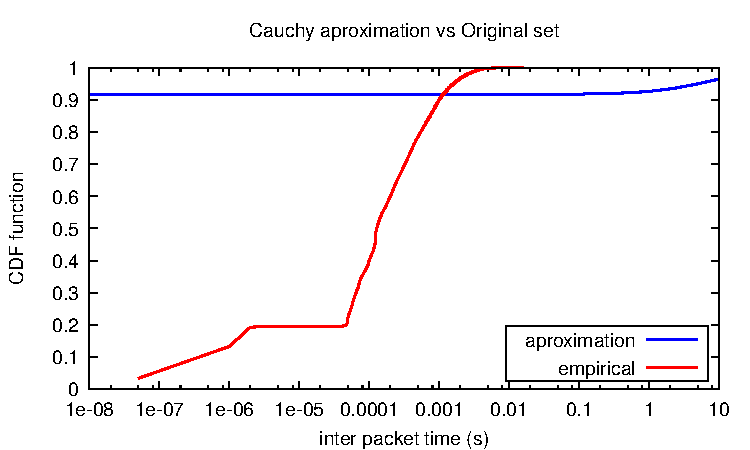
\includegraphics[width=78mm]{figures/apC/cdf/bigFlows_Logscale_-_Cauchy_aproximation_vs_Original_set}
	}
	\subfloat[Exponential(LR)]{
		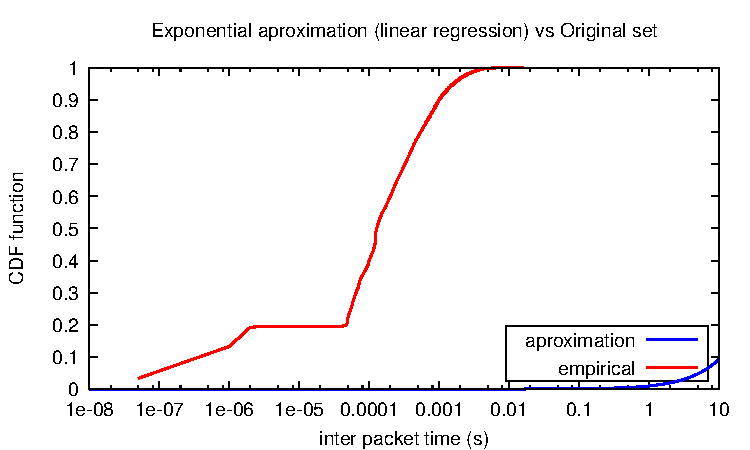
\includegraphics[width=78mm]{figures/apC/cdf/bigFlows_Logscale_-_Exponential_aproximation_(linear_regression)_vs_Original_set}
	}
	\hspace{0mm}
	\subfloat[Exponential(Me)]{
		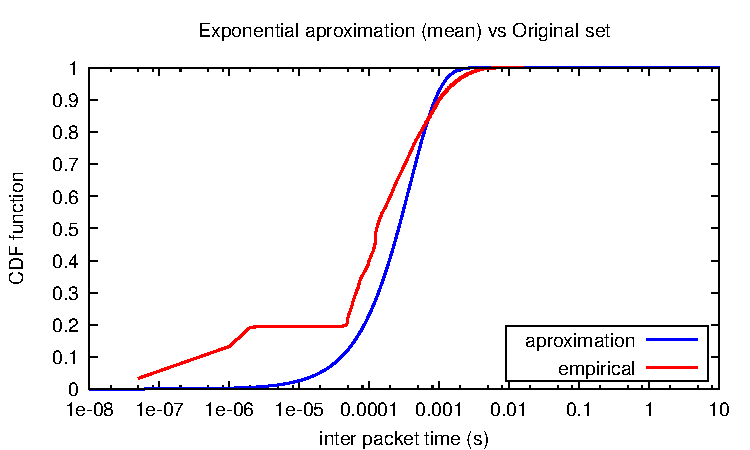
\includegraphics[width=78mm]{figures/apC/cdf/bigFlows_Logscale_-_Exponential_aproximation_(mean)_vs_Original_set}
	}
	\subfloat[Normal]{
		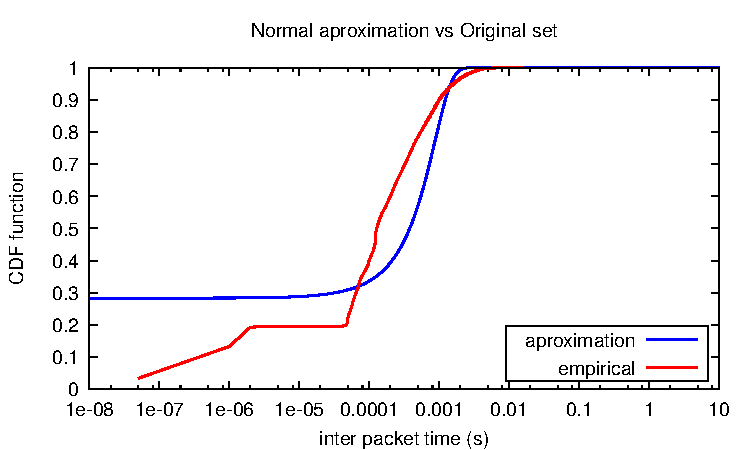
\includegraphics[width=78mm]{figures/apC/cdf/bigFlows_Logscale_-_Normal_aproximation_vs_Original_set}
	}
	\hspace{0mm}
	\subfloat[Pareto(LR)]{
		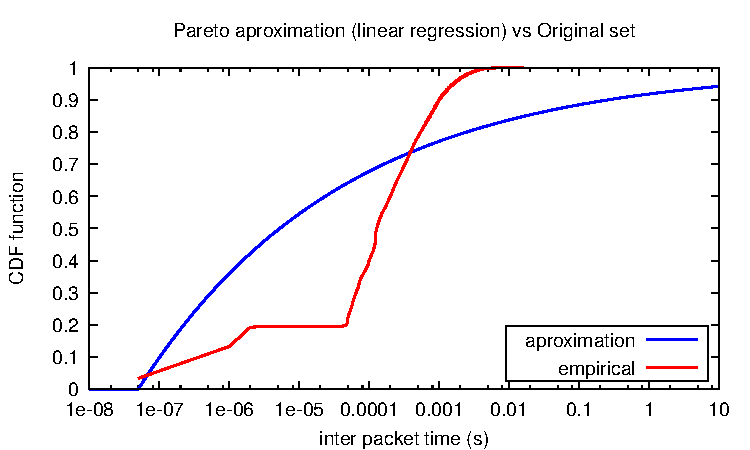
\includegraphics[width=78mm]{figures/apC/cdf/bigFlows_Logscale_-_Pareto_aproximation_(linear_regression)_vs_Original_set}
	}
	\subfloat[Pareto(MLH)]{
		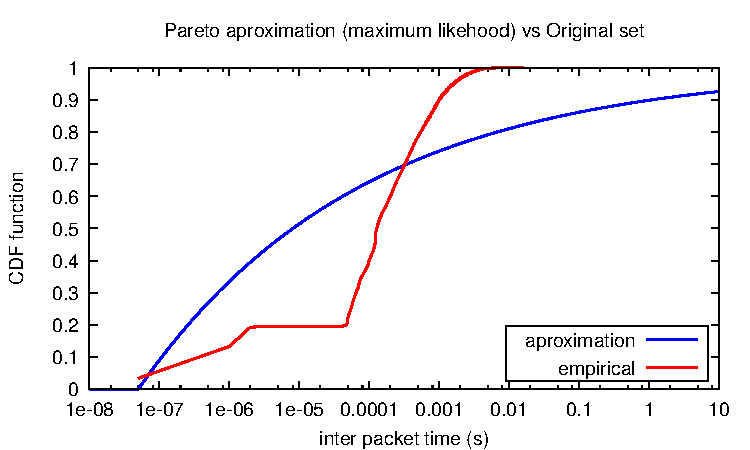
\includegraphics[width=78mm]{figures/apC/cdf/bigFlows_Logscale_-_Pareto_aproximation_(maximum_likehood)_vs_Original_set}
	}
	\hspace{0mm}
	\subfloat[Weibull]{
		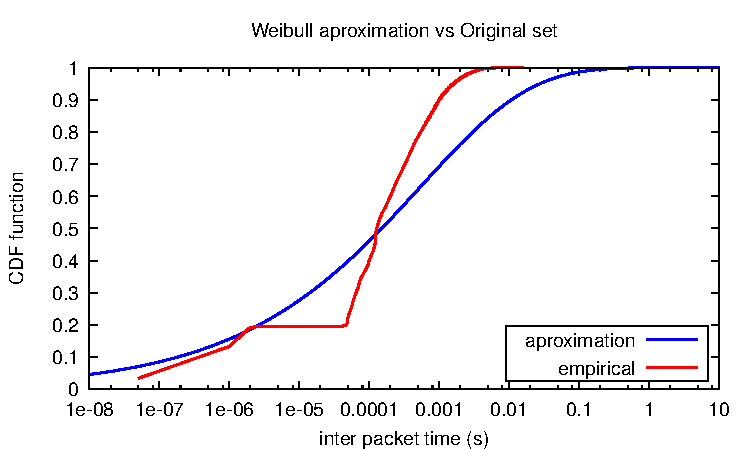
\includegraphics[width=78mm]{figures/apC/cdf/bigFlows_Logscale_-_Weibull_aproximation_vs_Original_set}
	}
	\caption{CDF functions for the approximations of \textit{bigFlows-pcap} inter  packet times, of many stochastic functions.}
\end{figure}

\begin{figure}[ht!]
	\centering
	\label{fig:aproximation-original-cdf-wan}
	\subfloat[Chauchy]{
		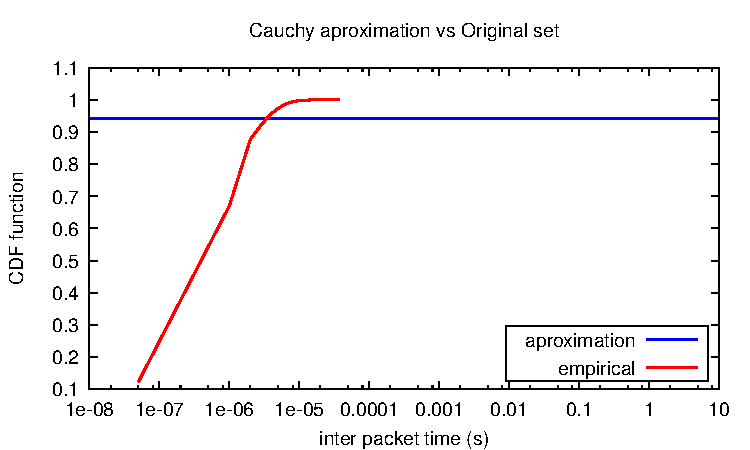
\includegraphics[width=78mm]{figures/apC/cdf/wan_Logscale_-_Cauchy_aproximation_vs_Original_set}
	}
	\subfloat[Exponential(LR)]{
		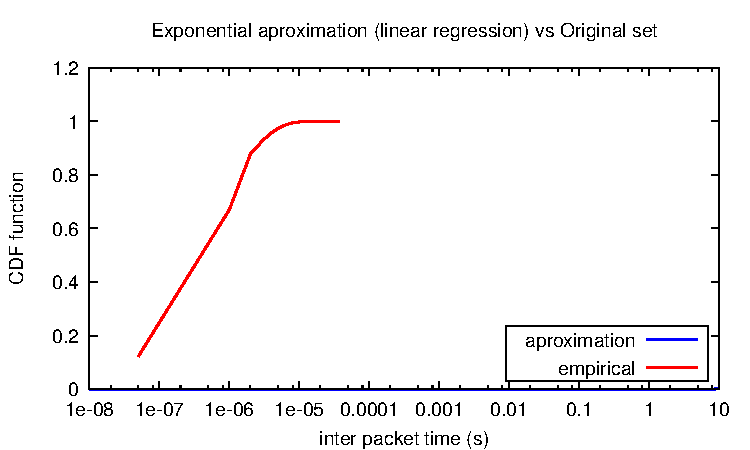
\includegraphics[width=78mm]{figures/apC/cdf/wan_Logscale_-_Exponential_aproximation_(linear_regression)_vs_Original_set}
	}
	\hspace{0mm}
	\subfloat[Exponential(Me)]{
		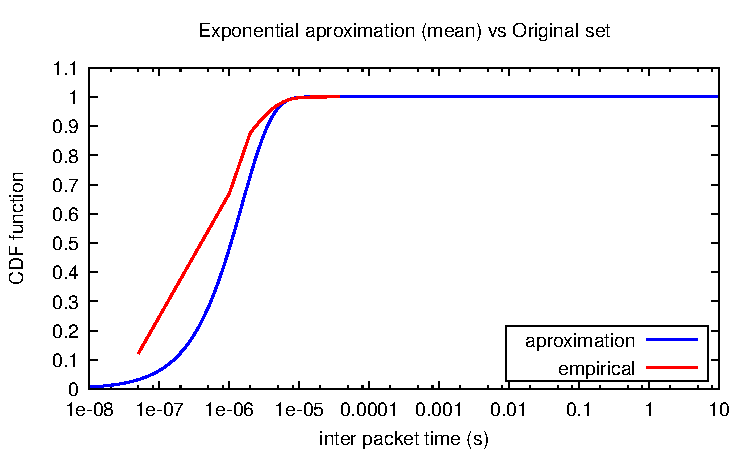
\includegraphics[width=78mm]{figures/apC/cdf/wan_Logscale_-_Exponential_aproximation_(mean)_vs_Original_set}
	}
	\subfloat[Normal]{
		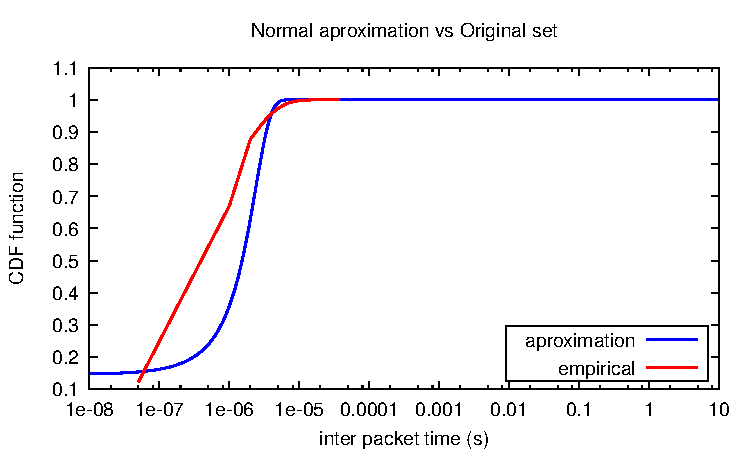
\includegraphics[width=78mm]{figures/apC/cdf/wan_Logscale_-_Normal_aproximation_vs_Original_set}
	}
	\hspace{0mm}
	\subfloat[Pareto(LR)]{
		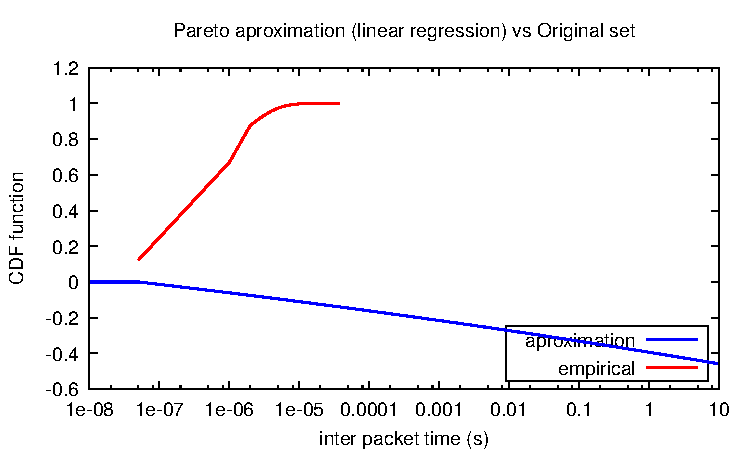
\includegraphics[width=78mm]{figures/apC/cdf/wan_Logscale_-_Pareto_aproximation_(linear_regression)_vs_Original_set}
	}
	\subfloat[Pareto(MLH)]{
		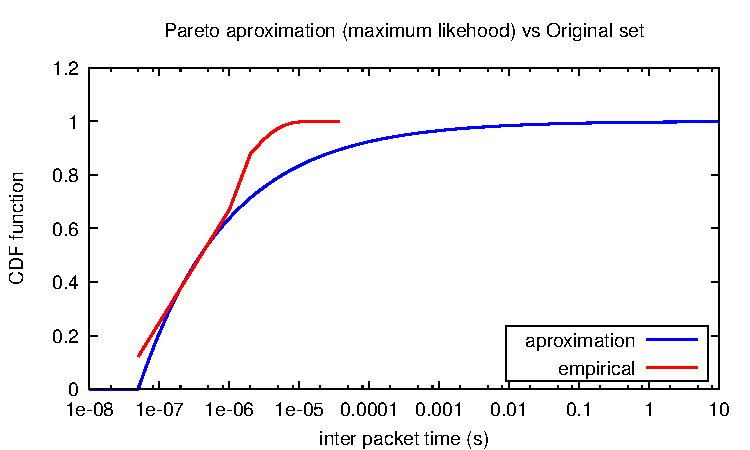
\includegraphics[width=78mm]{figures/apC/cdf/wan_Logscale_-_Pareto_aproximation_(maximum_likehood)_vs_Original_set}
	}
	\hspace{0mm}
	\subfloat[Weibull]{
		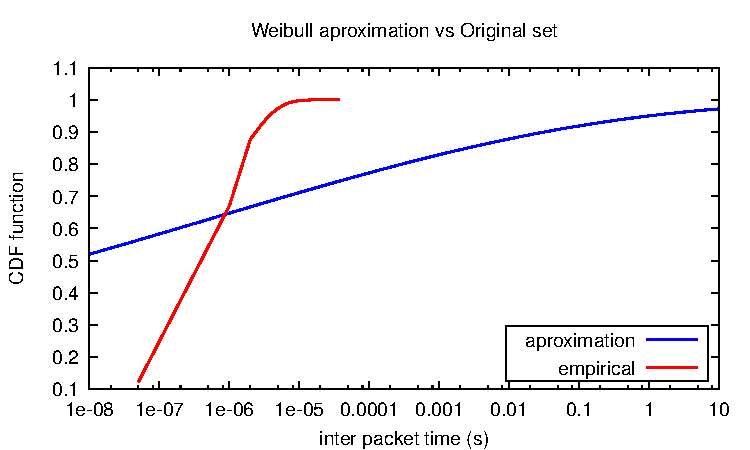
\includegraphics[width=78mm]{figures/apC/cdf/wan_Logscale_-_Weibull_aproximation_vs_Original_set}
	}
	\caption{CDF functions for the approximations of \textit{wan-pcap} inter  packet times, of many stochastic functions.}
\end{figure}


\begin{figure}[ht!]
	\centering
	\label{fig:aproximation-original-cdf-lan}
	\subfloat[Chauchy]{
		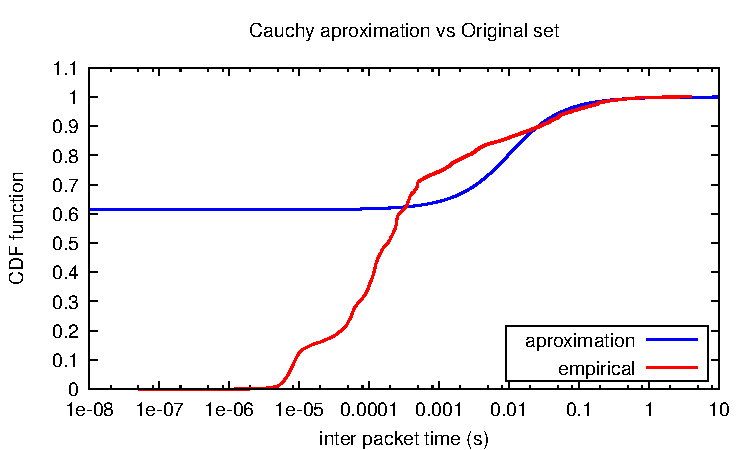
\includegraphics[width=78mm]{figures/apC/cdf/lan_Logscale_-_Cauchy_aproximation_vs_Original_set}
	}
	\subfloat[Exponential(LR)]{
		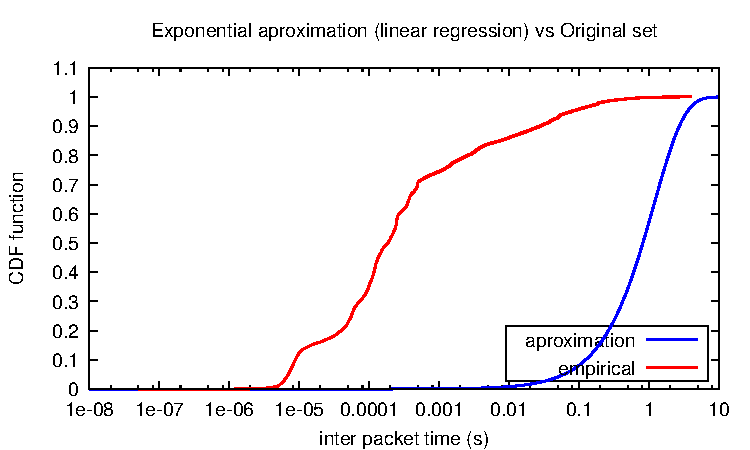
\includegraphics[width=78mm]{figures/apC/cdf/lan_Logscale_-_Exponential_aproximation_(linear_regression)_vs_Original_set}
	}
	\hspace{0mm}
	\subfloat[Exponential(Me)]{
		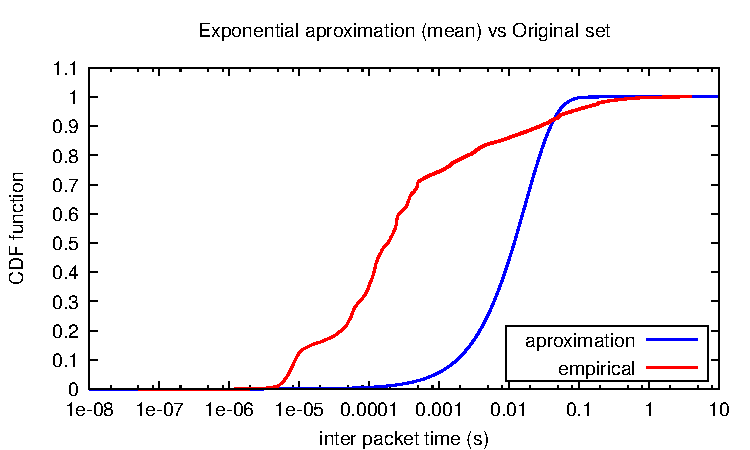
\includegraphics[width=78mm]{figures/apC/cdf/lan_Logscale_-_Exponential_aproximation_(mean)_vs_Original_set}
	}
	\subfloat[Normal]{
		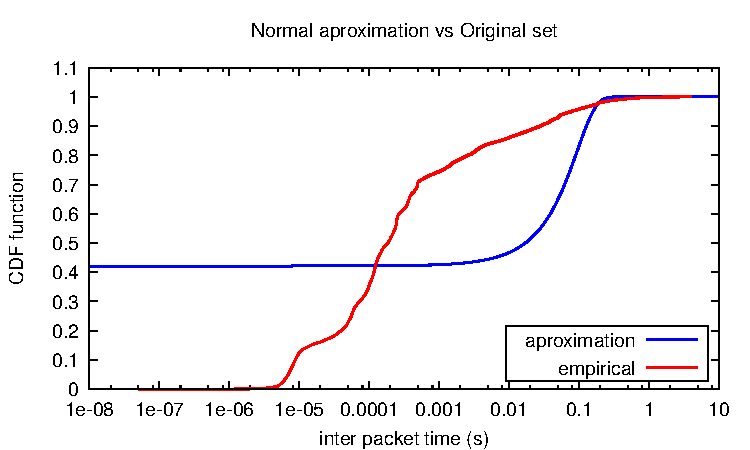
\includegraphics[width=78mm]{figures/apC/cdf/lan_Logscale_-_Normal_aproximation_vs_Original_set}
	}
	\hspace{0mm}
	\subfloat[Pareto(LR)]{
		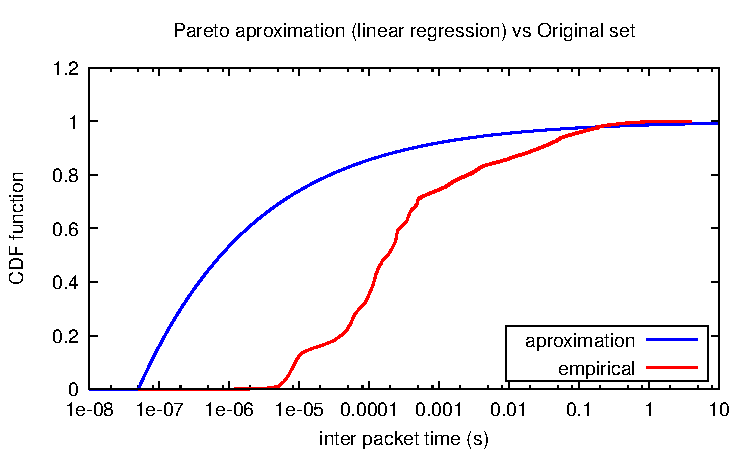
\includegraphics[width=78mm]{figures/apC/cdf/lan_Logscale_-_Pareto_aproximation_(linear_regression)_vs_Original_set}
	}
	\subfloat[Pareto(MLH)]{
		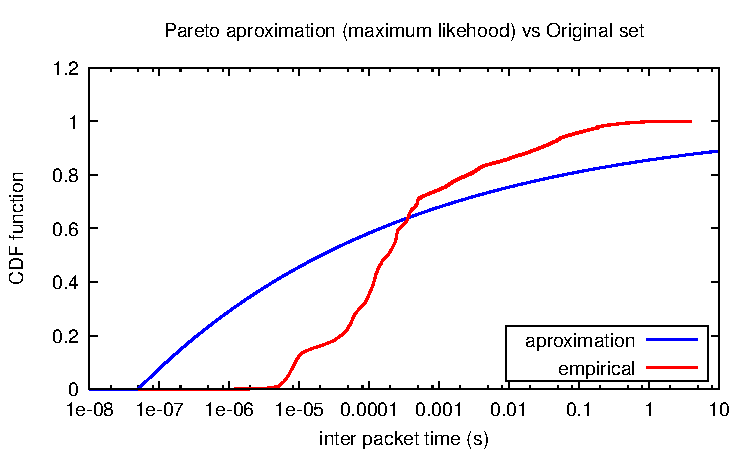
\includegraphics[width=78mm]{figures/apC/cdf/lan_Logscale_-_Pareto_aproximation_(maximum_likehood)_vs_Original_set}
	}
	\hspace{0mm}
	\subfloat[Weibull]{
		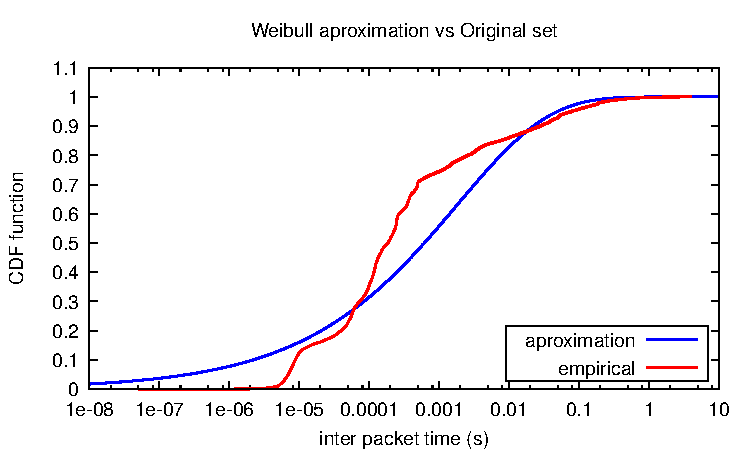
\includegraphics[width=78mm]{figures/apC/cdf/lan_Logscale_-_Weibull_aproximation_vs_Original_set}
	}
	\caption{CDF functions for the approximations of \textit{lan-diurnal-pcap} inter  packet times, of many stochastic functions.}
\end{figure}


\section{QQplots}

%\begin{figure}[ht!]
%	\centering
%	\label{fig:aproximation-original-cdf-skype}
%	\subfloat[Chauchy]{
%		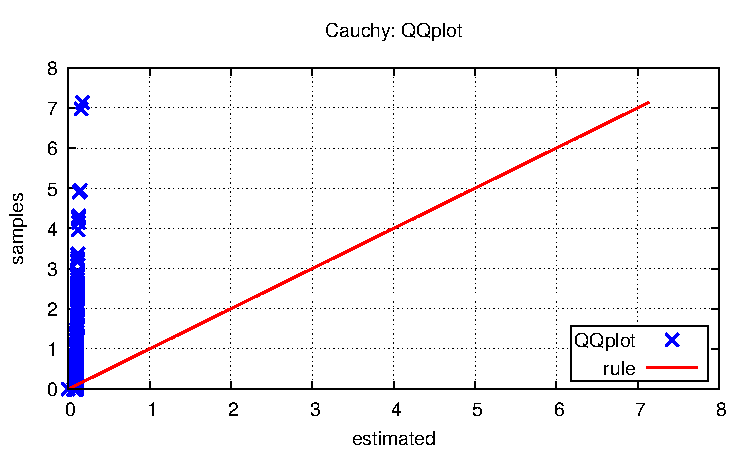
\includegraphics[width=78mm]{figures/apC/qq/skype_QQplot_-_Cauchy}
%	}
%	\subfloat[Exponential(LR)]{
%		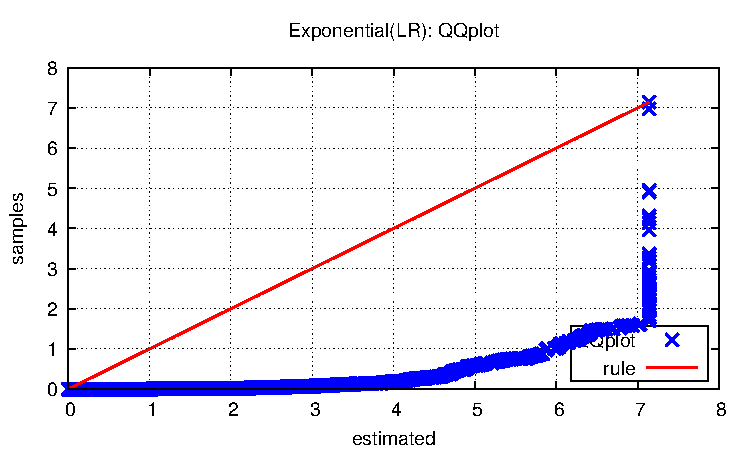
\includegraphics[width=78mm]{figures/apC/qq/skype_QQplot_-_Exponential(LR)}
%	}
%	\hspace{0mm}
%	\subfloat[Exponential(Me)]{
%		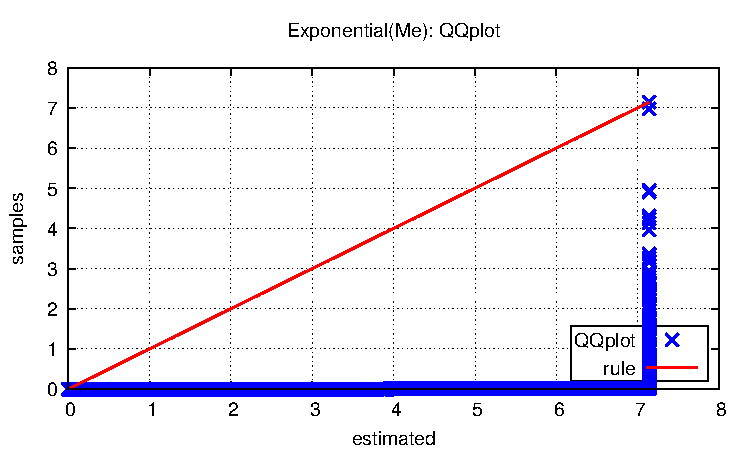
\includegraphics[width=78mm]{figures/apC/qq/skype_QQplot_-_Exponential(Me)}
%	}
%	\subfloat[Normal]{
%		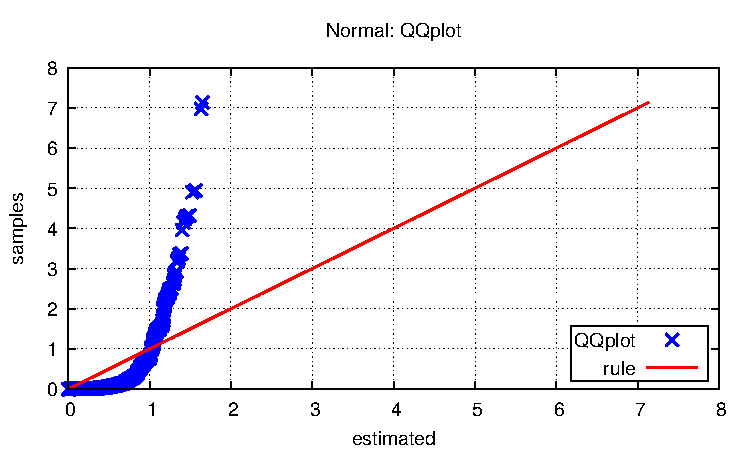
\includegraphics[width=78mm]{figures/apC/qq/skype_QQplot_-_Normal}
%	}
%	\hspace{0mm}
%	\subfloat[Pareto(LR)]{
%		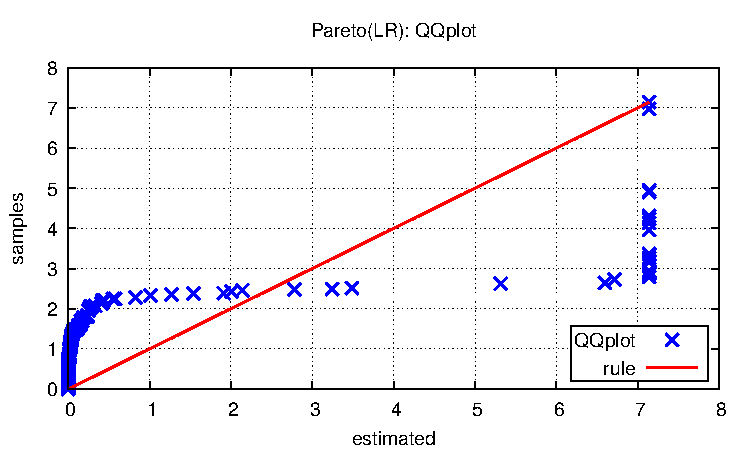
\includegraphics[width=78mm]{figures/apC/qq/skype_QQplot_-_Pareto(LR)}
%	}
%	\subfloat[Pareto(MLH)]{
%		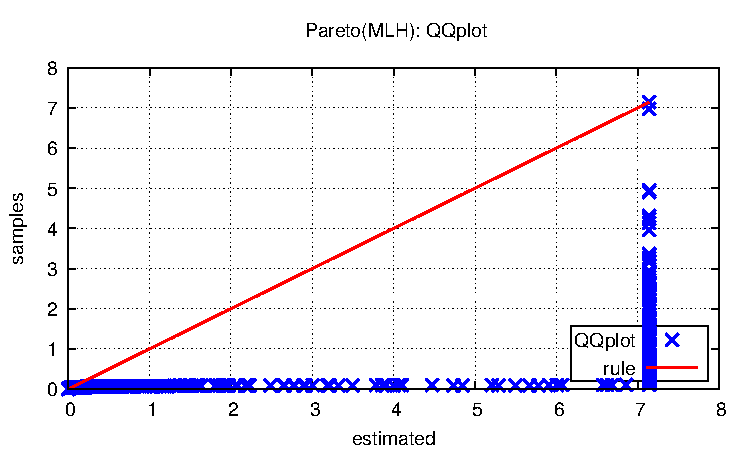
\includegraphics[width=78mm]{figures/apC/qq/skype_QQplot_-_Pareto(MLH)}
%	}
%	\hspace{0mm}
%	\subfloat[Weibull]{
%		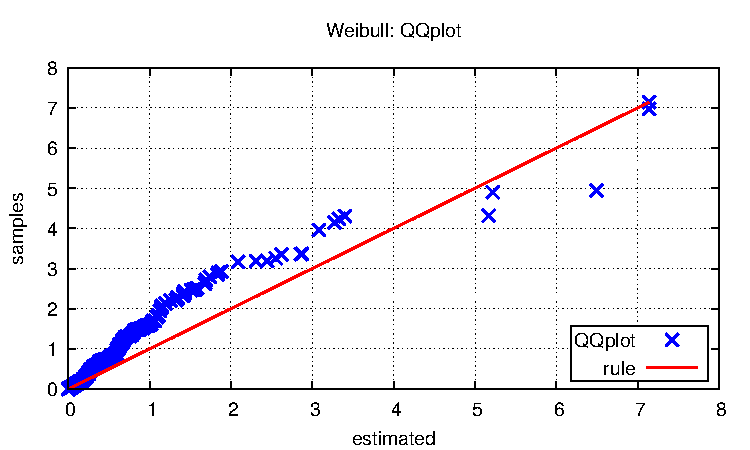
\includegraphics[width=78mm]{figures/apC/qq/skype_QQplot_-_Weibull}
%	}
%	\caption{CDF functions for the approximations of \textit{skype-pcap} inter  packet times, of many stochastic functions.}
%\end{figure}


\begin{figure}[ht!]
	\centering
	\label{fig:qq-bigFlows}
	\subfloat[Chauchy]{
		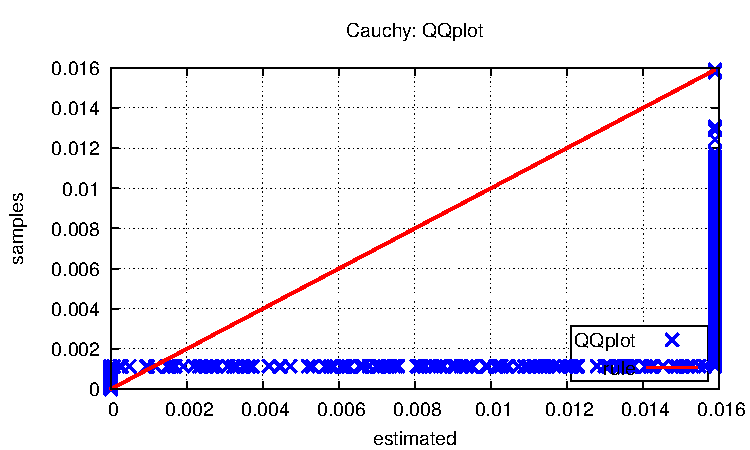
\includegraphics[width=78mm]{figures/apC/qq/bigFlows_QQplot_-_Cauchy}
	}
	\subfloat[Exponential(LR)]{
		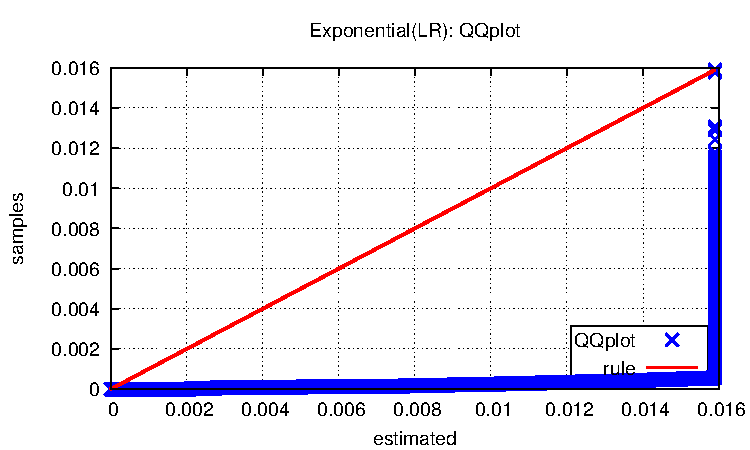
\includegraphics[width=78mm]{figures/apC/qq/bigFlows_QQplot_-_Exponential(LR)}
	}
	\hspace{0mm}
	\subfloat[Exponential(Me)]{
		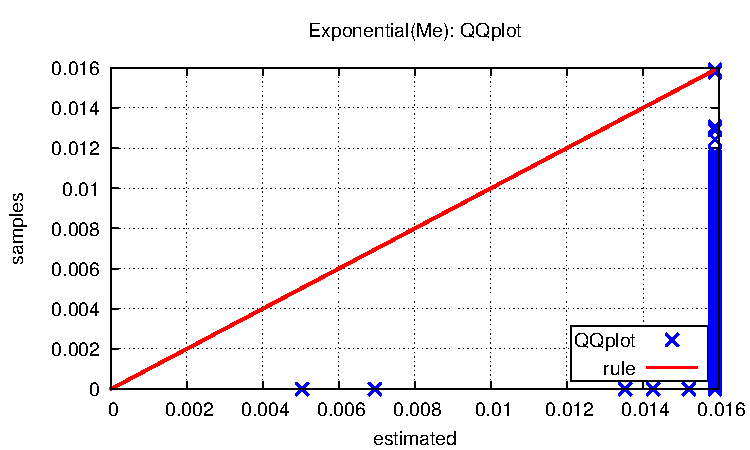
\includegraphics[width=78mm]{figures/apC/qq/bigFlows_QQplot_-_Exponential(Me)}
	}
	\subfloat[Normal]{
		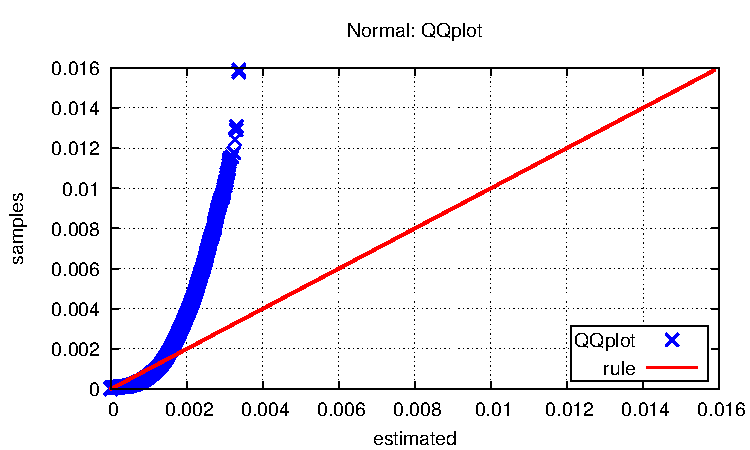
\includegraphics[width=78mm]{figures/apC/qq/bigFlows_QQplot_-_Normal}
	}
	\hspace{0mm}
	\subfloat[Pareto(LR)]{
		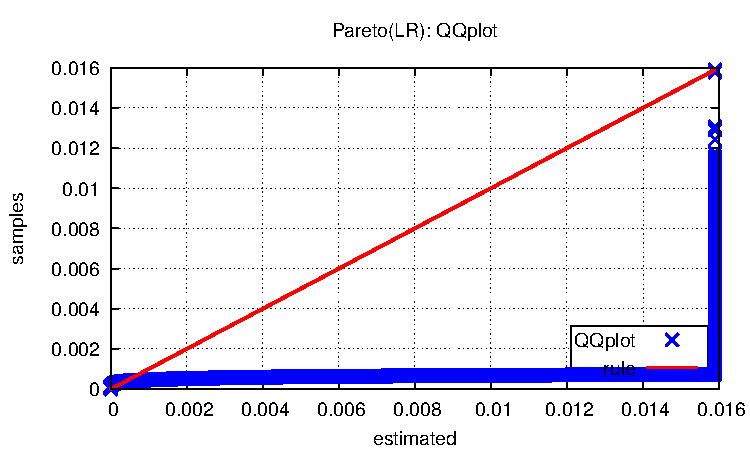
\includegraphics[width=78mm]{figures/apC/qq/bigFlows_QQplot_-_Pareto(LR)}
	}
	\subfloat[Pareto(MLH)]{
		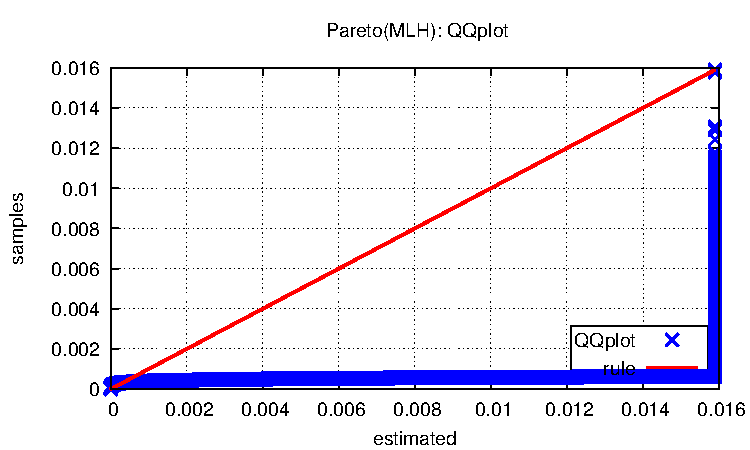
\includegraphics[width=78mm]{figures/apC/qq/bigFlows_QQplot_-_Pareto(MLH)}
	}
	\hspace{0mm}
	\subfloat[Weibull]{
		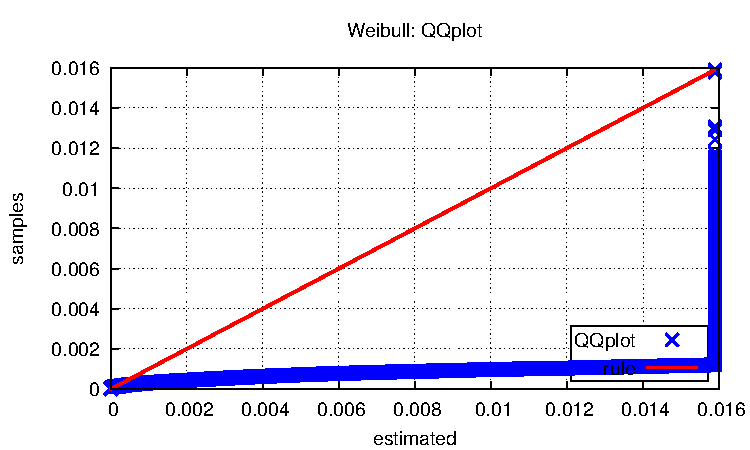
\includegraphics[width=78mm]{figures/apC/qq/bigFlows_QQplot_-_Weibull}
	}
	\caption{CDF functions for the approximations of \textit{bigFlows-pcap} inter  packet times, of many stochastic functions.}
\end{figure}



\begin{figure}[ht!]
	\centering
	\label{fig:qq-lan}
	\subfloat[Chauchy]{
		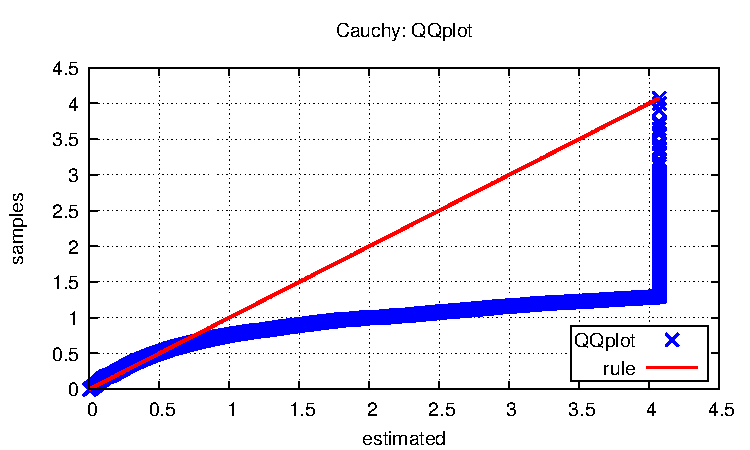
\includegraphics[width=78mm]{figures/apC/qq/lan_QQplot_-_Cauchy}
	}
	\subfloat[Exponential(LR)]{
		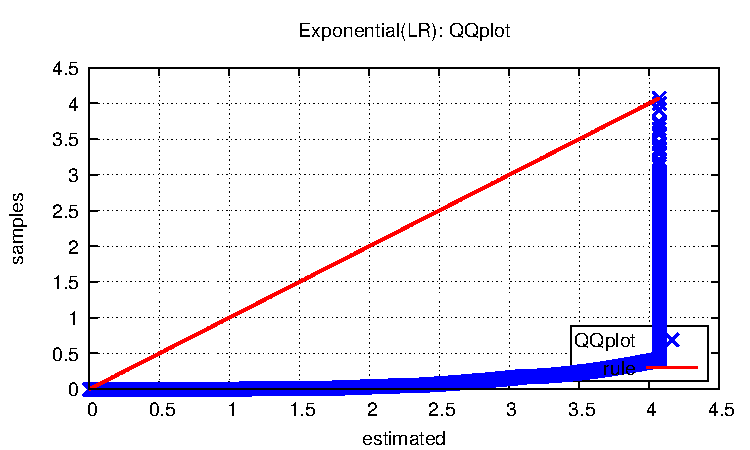
\includegraphics[width=78mm]{figures/apC/qq/lan_QQplot_-_Exponential(LR)}
	}
	\hspace{0mm}
	\subfloat[Exponential(Me)]{
		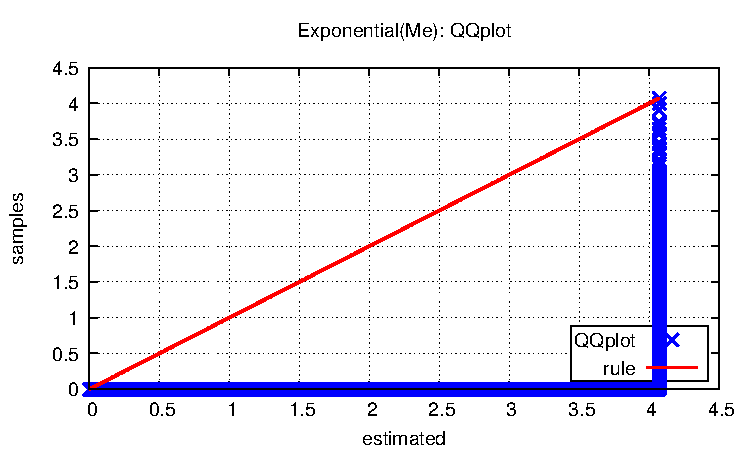
\includegraphics[width=78mm]{figures/apC/qq/lan_QQplot_-_Exponential(Me)}
	}
	\subfloat[Normal]{
		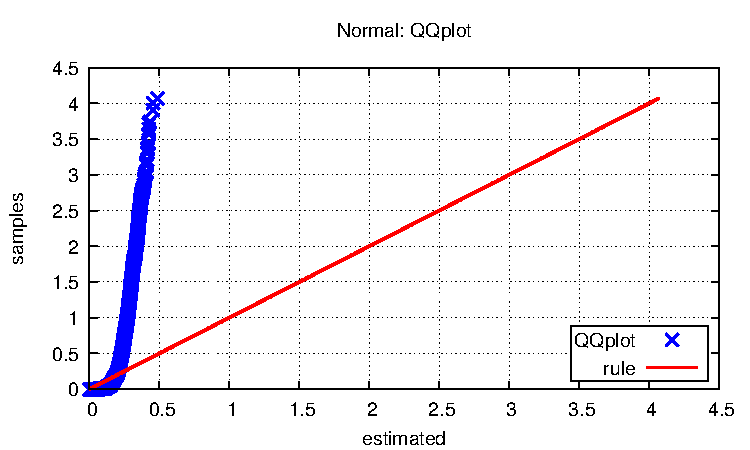
\includegraphics[width=78mm]{figures/apC/qq/lan_QQplot_-_Normal}
	}
	\hspace{0mm}
	\subfloat[Pareto(LR)]{
		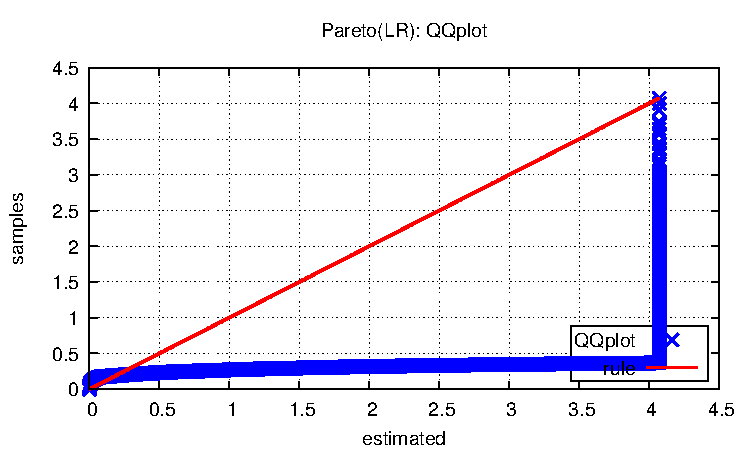
\includegraphics[width=78mm]{figures/apC/qq/lan_QQplot_-_Pareto(LR)}
	}
	\subfloat[Pareto(MLH)]{
		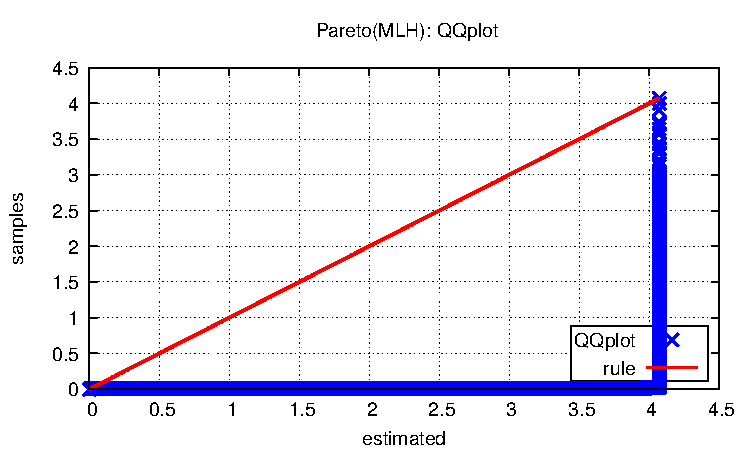
\includegraphics[width=78mm]{figures/apC/qq/lan_QQplot_-_Pareto(MLH)}
	}
	\hspace{0mm}
	\subfloat[Weibull]{
		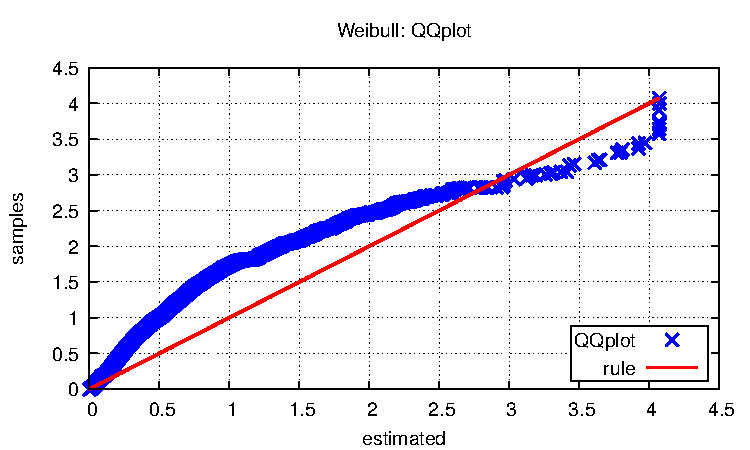
\includegraphics[width=78mm]{figures/apC/qq/lan_QQplot_-_Weibull}
	}
	\caption{CDF functions for the approximations of \textit{lan-diurnal-pcap} inter  packet times, of many stochastic functions.}
\end{figure}



\begin{figure}[ht!]
	\centering
	\label{fig:qq-wan}
	\subfloat[Chauchy]{
		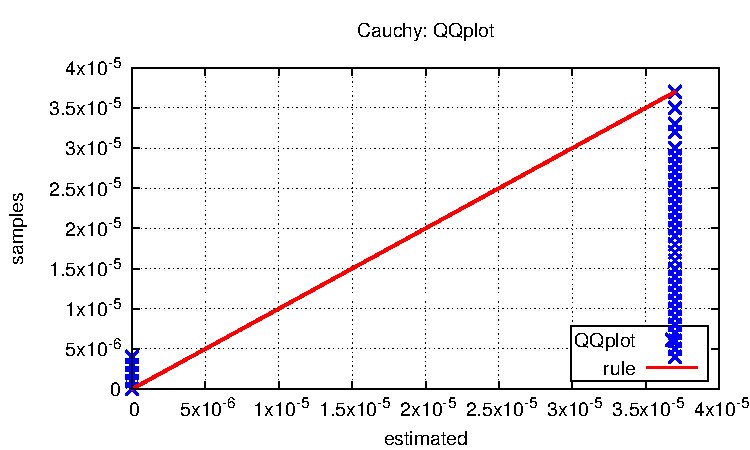
\includegraphics[width=78mm]{figures/apC/qq/wan_QQplot_-_Cauchy}
	}
	\subfloat[Exponential(LR)]{
		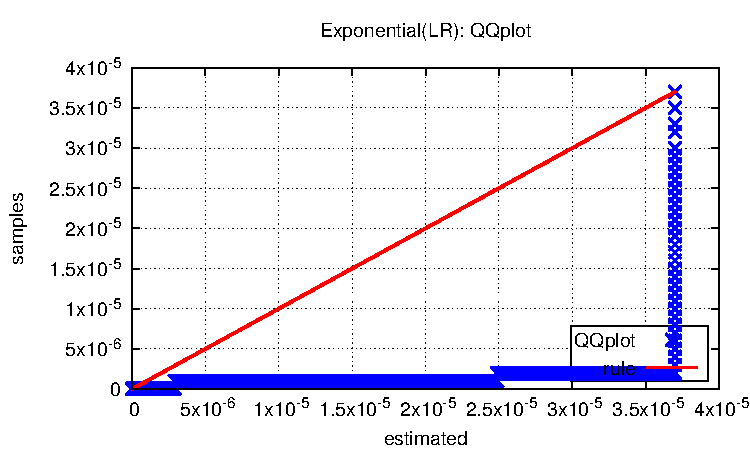
\includegraphics[width=78mm]{figures/apC/qq/wan_QQplot_-_Exponential(LR)}
	}
	\hspace{0mm}
	\subfloat[Exponential(Me)]{
		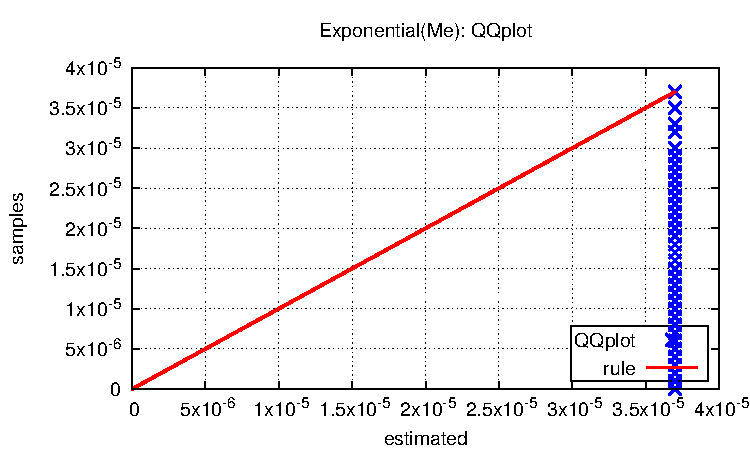
\includegraphics[width=78mm]{figures/apC/qq/wan_QQplot_-_Exponential(Me)}
	}
	\subfloat[Normal]{
		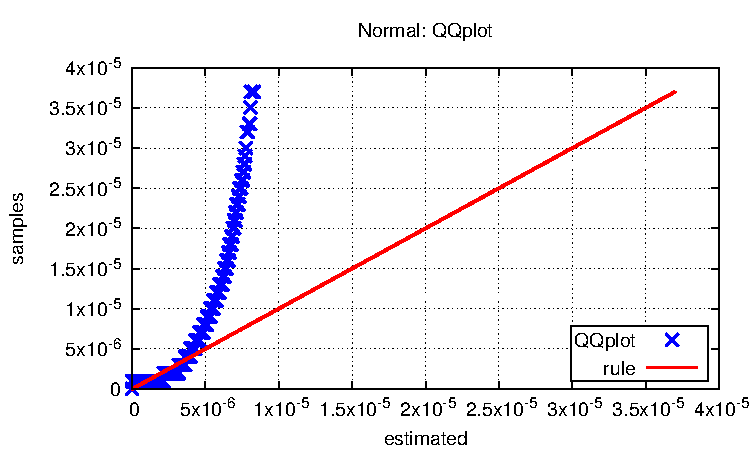
\includegraphics[width=78mm]{figures/apC/qq/wan_QQplot_-_Normal}
	}
	\hspace{0mm}
	\subfloat[Pareto(LR)]{
		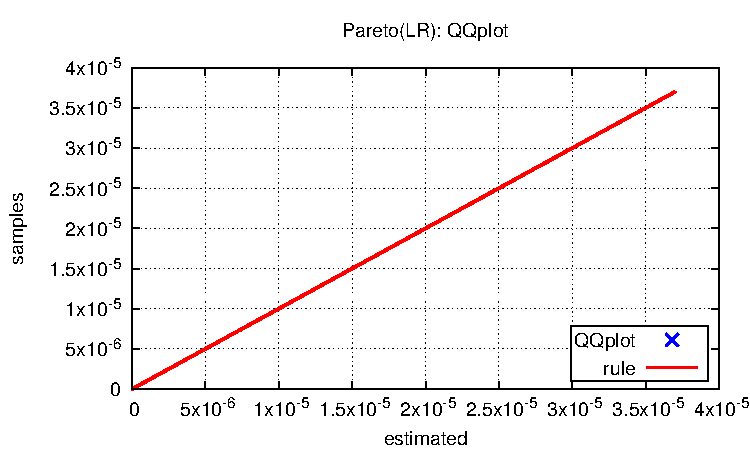
\includegraphics[width=78mm]{figures/apC/qq/wan_QQplot_-_Pareto(LR)}
	}
	\subfloat[Pareto(MLH)]{
		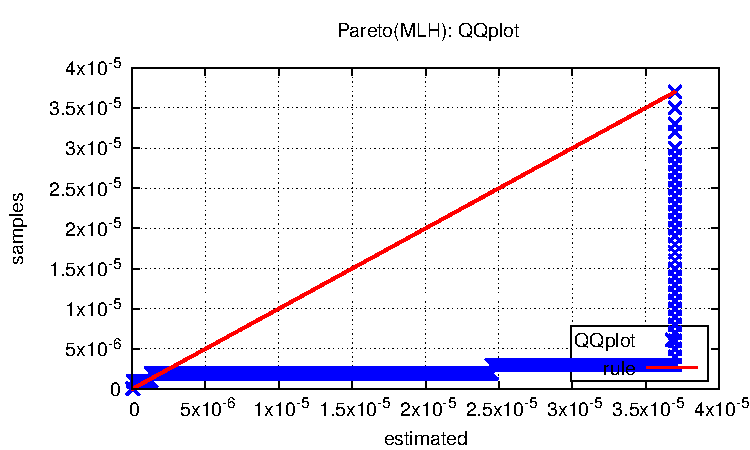
\includegraphics[width=78mm]{figures/apC/qq/wan_QQplot_-_Pareto(MLH)}
	}
	\hspace{0mm}
	\subfloat[Weibull]{
		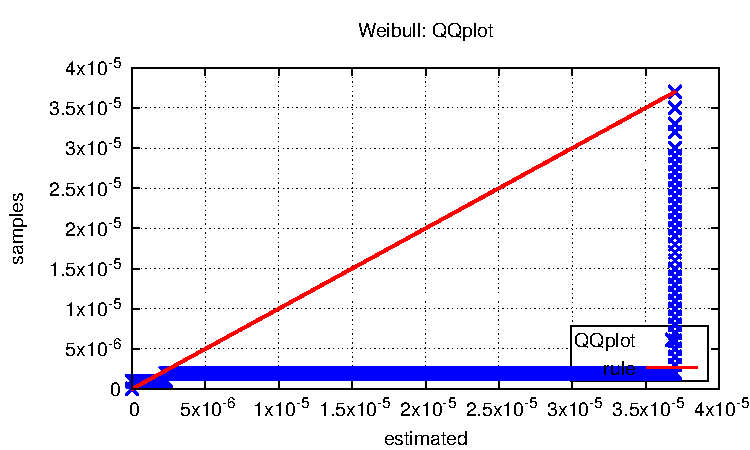
\includegraphics[width=78mm]{figures/apC/qq/wan_QQplot_-_Weibull}
	}
	\caption{CDF functions for the approximations of \textit{wan-pcap} inter  packet times, of many stochastic functions.}
\end{figure}


\section{Validation}




\begin{figure}[ht!]
	\centering
	\label{fig:correlation-hurst-bigflows}
	\subfloat[]{
		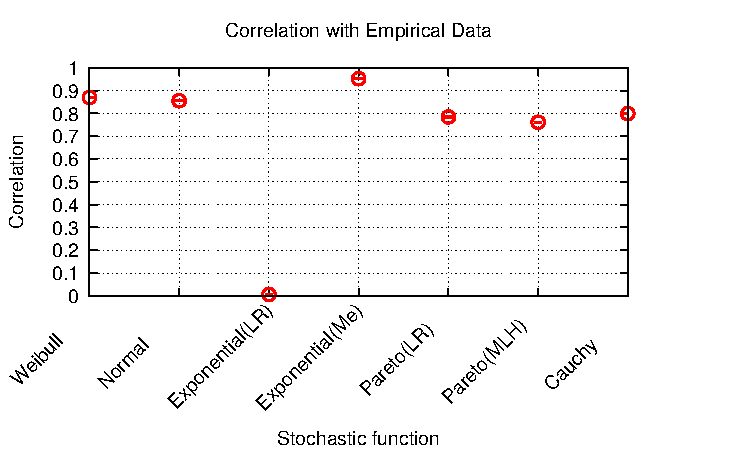
\includegraphics[width=75mm]{figures/apC/val/bigFlows_Correlation}
		\label{correlation-skype-pcap}
	}
	\hspace{0mm}
	\subfloat[]{
		\includegraphics[width=75mm]{figures/apC/val/bigFlows_Hurst_Exponent}
	}
	\hspace{0mm}
	\subfloat[]{
		\includegraphics[width=75mm]{figures/apC/val/bigFlows_Mean}
	}
	\hspace{0mm}
	\subfloat[]{
		\includegraphics[width=75mm]{figures/apC/val/bigFlows_Standard_Deviation}
		\label{hurst-skype-pcap}
	}
	\caption{Statistical parameters of \textit{bigflows-pcap} and its approximations}
\end{figure}

\begin{figure}[ht!]
	\centering
	\label{fig:correlation-hurst-lan}
	\subfloat[]{
		\includegraphics[width=75mm]{figures/apC/val/lan_Correlation}
		\label{correlation-skype-pcap}
	}
	\hspace{0mm}
	\subfloat[]{
		\includegraphics[width=75mm]{figures/apC/val/lan_Hurst_Exponent}
	}
	\hspace{0mm}
	\subfloat[]{
		\includegraphics[width=75mm]{figures/apC/val/lan_Mean}
	}
	\hspace{0mm}
	\subfloat[]{
		\includegraphics[width=75mm]{figures/apC/val/lan_Standard_Deviation}
		\label{hurst-skype-pcap}
	}
	\caption{Statistical parameters of \textit{lan-diurnal-pcap} and its approximations}
\end{figure}


\begin{figure}[ht!]
	\centering
	\label{fig:correlation-hurst-wan}
	\subfloat[]{
		\includegraphics[width=75mm]{figures/apC/val/wan_Correlation}
		\label{correlation-skype-pcap}
	}
	\hspace{0mm}
	\subfloat[]{
		\includegraphics[width=75mm]{figures/apC/val/wan_Hurst_Exponent}
	}
	\hspace{0mm}
	\subfloat[]{
		\includegraphics[width=75mm]{figures/apC/val/wan_Mean}
	}
	\hspace{0mm}
	\subfloat[]{
		\includegraphics[width=75mm]{figures/apC/val/wan_Standard_Deviation}
		\label{hurst-skype-pcap}
	}
	\caption{Statistical parameters of \textit{wan-pcap} and its approximations}
\end{figure}






